\documentclass[12pt]{article}
\usepackage{amsmath}
\usepackage{mathtools}
\usepackage{bigints}
\usepackage{parskip}
\usepackage{amssymb}
\usepackage{relsize}
\usepackage{fullpage}
% \DeclareMathSizes{12}{17.28}{9}{7} % (a)

\DeclareMathSizes{12}{17.28}{12}{12} % (a)


\usepackage{hyperref}



	\addtolength{\topmargin}{-.5in}
	\addtolength{\textheight}{1.75in}



    \newenvironment{myindentpar}[1]%
     {\begin{list}{}%
             {\setlength{\leftmargin}{#1}}%
             \item[]%
     }
     {\end{list}}

\begin{document}
\title{College Algebra: Module 8 What You Need To Know}
\date{2-26-15}
\author{}
\maketitle


\section{Functions, Function Notation, and the Graph of a Function (Section 2.4)}

\textbf{Function} - a \textit{function} is a set of ordered pairs $(x,y)$ in which each first coordinate is paired with only one second coordinate

\textbf{Vertical Line Test:} - a nice, easy, graphical test to determine if a graph is a function. It says that a graph of an equation is a function if every vertical line intersects the graph \textbf{in at most one point.}

\begin{myindentpar}{1cm}

\textbf{Graph That Passes the Vertical Line Test:}

\centerline{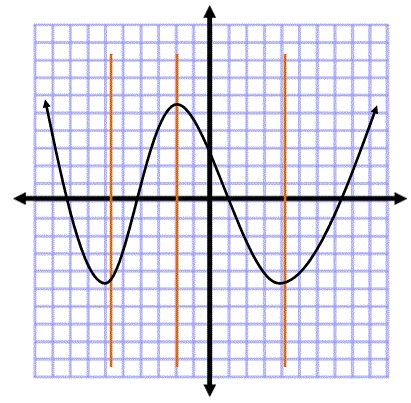
\includegraphics{PassesVLT.jpg}}

\newpage

\textbf{Graph That Fails the Vertical Line Test:}

\centerline{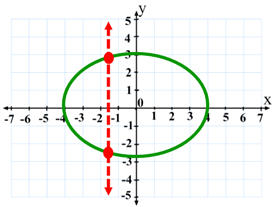
\includegraphics{FailsVLT.jpg}}

\end{myindentpar}

\textbf{Domain} - the set of numbers that you can input into your function

\begin{myindentpar}{1cm}
\textbf{Note:} Usually you need to be careful of two types of functions: 

\begin{enumerate}
\item \textbf{Finding the Domain of the Square Root Function: $f(x) = \sqrt{x}$} 

If you have a function of the form $\sqrt{STUFF}$ you then solve the inequality 
\newline

\centerline{$STUFF \geq 0$}

to find the domain of the function.


\item \textbf{Finding the Domain of a Rational Function:  $f(x) = \dfrac{P(x)}{R(x)}$}

 A rational function is of the form $f(x) = \dfrac{P(x)}{R(x)}$ where $P(x)$ and $R(x)$ are polynomial. The domain of a rational function is all reals except for $R(x)=0.$ 

What this means is that to find the domain of a rational function you \textbf{set the denominator equal to 0 and solve that}. You then \textbf{exclude} those values from the domain of your function.
\end{enumerate}

 \textbf{Note:} Sometimes you might see a combination of both. For example, find the domain of $f(x) = \dfrac{-1}{\sqrt{x+8}}$. We do this by solving $x+8>0$
\end{myindentpar}

Graphically, you can determine the domain by scanning along the x-axis and seeing what x-values the function is not defined for.

\textbf{Range} - the set of numbers that are output from a function. Often harder to determine than the domain, we can determine the range graphically by scanning along the y-axis and seeing what y-values the function is not defined for.

\section{Analyzing the Graph of a Function (Section 2.5)}

{\bf \underline{Even \& Odd Functions}}
\begin{myindentpar}{1cm}
\textbf{Even Function} - a function is \textit{even} if $f(-x) = f(x)$ Even functions are always symmetric about the y-axis.

\textbf{Odd Function} - a function is \textit{odd} if $f(-x) = -f(x)$ Odd functions are always symmetric about the origin.
\end{myindentpar}

\textbf{Increasing:} A function $f$ is \textit{increasing} on an interval $I$ if for any $x_{1}, x_{2}$ in $I$ with $x_{1} < x_{2} \implies f(x_{1}) < f(x_{2})$

\textbf{Decreasing:} A function $f$ is \textit{decreasing} on an interval $I$ if for any $x_{1}, x_{2}$ in $I$ with $x_{1} < x_{2} \implies f(x_{1}) > f(x_{2})$

\textbf{Constant:} A function $f$ is \textit{constant} on an interval $I$ if for all $x_{1}, x_{2}$ in $I \implies  f(x_{1}) = f(x_{2})$

\section{The Toolbox Functions and Transformations (Section 3.1)}

\subsection{Transformations}

\textbf{Vertical Shifts:} Let $c>0$

\begin{enumerate}
\item $y=f(x) + c$ shifts $f(x)$ c units up
\item $y=f(x) - c$ shifts $f(x)$ c units down
\end{enumerate}

\textbf{Horizontal Shifts:} Let $c>0$

\begin{enumerate}
\item $y=f(x+c)$ shifts $f(x)$ c units left
\item $y=f(x-c)$ shifts $f(x)$ c units right
\end{enumerate}

\textbf{Reflections:} 

\begin{enumerate}
\item $y=-f(x)$ reflects $f(x)$ about the x-axis
\item $y=f(-x)$ reflects $f(x)$ about the y-axis
\end{enumerate}

\textbf{Vertical Stretch \& Shrink:} 
\newline

\centerline{Let $c>0$. We consider $y=cf(x)$}

\begin{enumerate}
\item $c>1 \hspace{1.1cm} \to$ stretch $f(x)$ vertically by a factor of c
\item $0<c<1 \to$ shrink $f(x)$ vertically by a factor of c
\end{enumerate}
\vspace{.5cm}
\textbf{Horizontal Stretch \& Shrink:} 
\newline

\centerline{Let $c>0$. We consider $y=f(cx)$}

\begin{enumerate}
\item $c>1 \hspace{1.1cm} \to$ shrink $f(x)$ horizontally by a factor of c
\item $0<c<1 \to$ stretch $f(x)$ horizontally by a factor of c
\end{enumerate}

\newpage

\textbf{Order of Transformations:}

\begin{enumerate}

\item Horizontal Shift 
\item Stretch/Shrink 
\item Reflections
\item Vertical Shift

\end{enumerate}

\textbf{Graphs of Common Functions with Their Domain and Range}

\textbf{Graph of Quadratic Function $\mathbf{y=x^2}$}

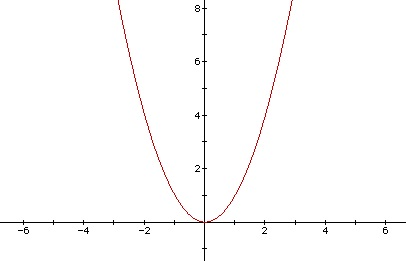
\includegraphics{Quadratic.jpg}

\textbf{Domain:} $(-\infty, \infty)$ \hspace{2cm} \textbf{Range} $y \geq 0$

\textbf{Graph of Cubic Function $\mathbf{y=x^3}$}

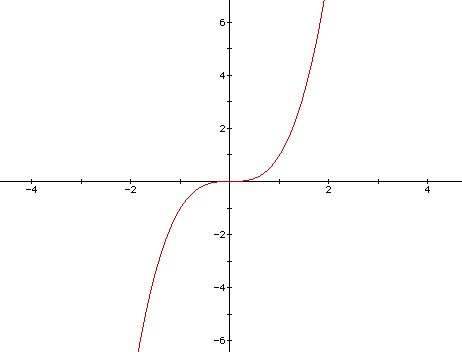
\includegraphics[scale = 0.9]{CubeFunction.jpg}

\textbf{Domain:} $(-\infty, \infty)$ \hspace{2cm} \textbf{Range} $(-\infty, \infty)$

\newpage

\textbf{Graph of Absolute Value $\mathbf{y=|x|}$}

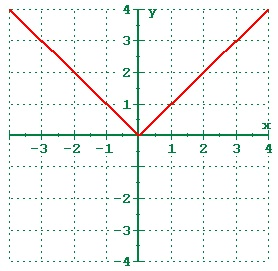
\includegraphics[scale = 0.9]{AbsoluteValue.jpg}

\textbf{Domain:} $(-\infty, \infty)$ \hspace{2cm} \textbf{Range} $y \geq 0$

\textbf{Graph of Square Root $\mathbf{y=\sqrt{x} = x^{1/2}}$}

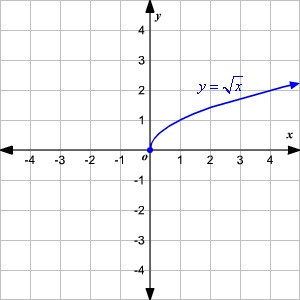
\includegraphics{SquareRoot.jpg}

\textbf{Domain:} $x \geq 0$ \hspace{2cm} \textbf{Range} $y \geq 0$

\newpage

\textbf{Graph of Cubic Root Function $\mathbf{y=\sqrt[3]{x} = x^{1/3}}$}

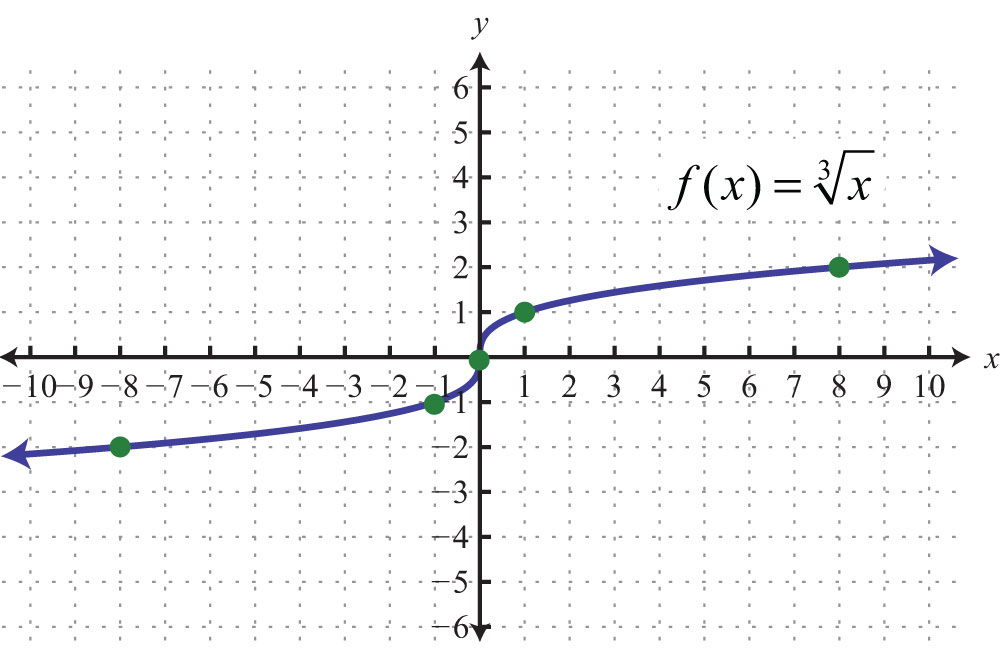
\includegraphics[scale = 0.3]{CubeRootFunction.jpg}

\textbf{Domain:} $(-\infty, \infty)$ \hspace{2cm} \textbf{Range} $(-\infty, \infty)$

\textbf{Graph of the Reciprocal Function $\mathbf{y=\dfrac{1}{x}}$}

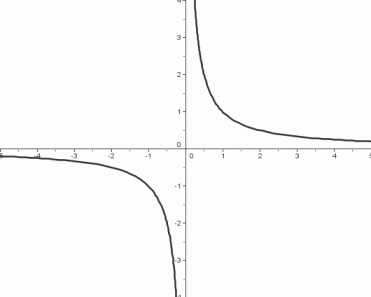
\includegraphics{RecipFunction.jpg}

\textbf{Domain:} $(-\infty, 0) \cup (0, \infty)$ \hspace{2cm} \textbf{Range} $(-\infty, 0) \cup (0, \infty)$ 




\end{document}